\section{Lógica de Reescrita} \label{sec:chap2}

Lógica de reescrita é definida como uma \textit{teoria de reescrita sortida} $\mathcal{R} = (\Sigma, E \cup B, R)$, onde $\Sigma$ é a sintaxe com \emph{sorts} da nossa teoria, $E$ é um conjunto de equações terminante e confluente, $B$ um conjunto de axiomas (e.g. associatividade, comutatividade e identidade) e $R$ é um conjunto de regras de reescrita no formato $t \rightarrow t'$ ou no formato condicional: $t \rightarrow t' \texttt{ se } \textbf{condição}$ \cite{RewritingLogicTwentyYears}. Assim, na representação de um sistema computacional utilizando a lógica de reescrita $\mathcal{R}$, a teoria equacional $(\Sigma, E \cup B)$ representa os estados do sistema como tipos de dados algébricos enquanto o conjunto de regras de reescrita $R$ (possivelmente não-confluente) especifica a dinâmica do sistema.

Devido a natureza não-determinística das regras de reescrita, onde qualquer regra de reescrita compatível com um determinado estado do sistema pode ser aplicada, sistemas concorrentes podem ser naturalmente modelados, devido a incerteza sobre a ordem de execução e comunicação entre os dispositivos. 
Por exemplo, considere um quarto com dispositivos inteligentes configurados para ligar o aquecedor quando a temperatura do quarto atingir 10ºC e ligar as luzes quando o horário for 18:30, e que, exatamente às 18:30 a temperatura chegou a 10ºC. Devido a natureza concorrente dos dispositivos, não é possível determinar qual ação ocorrerá primeiro: ligar as luzes ou ligar o aquecedor, mas é possível deduzir os cenários que podem ocorrer como um diagrama de transições:

\begin{figure}[h]
  \centering
  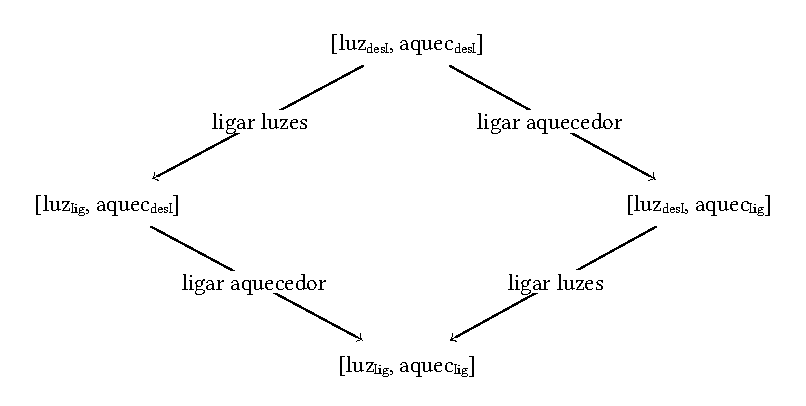
\includegraphics{img/diagram.pdf}
  \caption{Diagrama de transições}
  \label{fig:fig1}
\end{figure}

Este é um exemplo de situação confluente, onde todas as possibilidades de transições convergem para um mesmo estado, mas também existem situações não-confluentes, onde a ordem das transições pode resultar em estados divergentes.

\subsection{Maude} \label{sec:chap2sub1}

O software utilizado para a especificação do nosso modelo será o Maude, um framework em Lógica de Reescrita de alta performance.
No Maude, a sintaxe $\Sigma$ para construir sorts e operadores é definida utilizando o comando \texttt{op}, as equações $E$ utilizando o comando \texttt{eq}, e os axiomas $B$ são definidos como parâmetros no momento da declaração dos construtores utilizando o comando \texttt{op}.
O par $(\Sigma, E \cup B)$ no Maude deve definir funções totais, podendo serem vistas como programas funcionais.

Abaixo apresentamos uma definição de conjuntos de naturais no Maude para introduzir a sua sintaxe:

\begin{verbatim}
protecting NAT .
sort NatSet .
subsort Nat < NatSet .
\end{verbatim}

\noindent
Primeiro importamos um módulo do prelúdio, chamado \texttt{NAT}. \\
Definimos um sort chamado \texttt{NatSet} e especificamos que todo \texttt{N} também é um \texttt{NatSet}.

\begin{verbatim}
op empty : -> NatSet [ctor].
op _,_ : NatSet NatSet -> NatSet 
            [ctor assoc comm id: empty] .
\end{verbatim}

\noindent
Definimos um construtor de um \texttt{NatSet}, através de uma constante chamada \texttt{empty}. \\
Um construtor infixo posicional também é definido, que precisa de dois sorts \texttt{NatSet} para ser construído, onde \texttt{\_} indica as posições desses sorts no construtor. Este construtor também é definido como associativo, comutativo, e seu elemento identidade é \texttt{empty}.

\begin{verbatim}
var N : Nat .
var S : NatSet .

eq N,N = N .

op _in_ : Nat NatSet -> Bool .
eq N in (N,S) = true .
eq N in S = false [owise] .
\end{verbatim}

\noindent
Aqui definimos variáveis para utilizarmos nas nossas equações e operações. \\
A primeira equação faz com que nosso construtor de conjuntos seja idempotente. \\
Definimos uma operação para verificar se um elemento está num conjunto através de 2 equações parciais. A primeira equação utiliza \textit{pattern matching} para verificar se o elemento desejado está no conjunto, caso contrário, a segunda equação é aplicada.

Uma especificação no Maude pode ser dividida em módulos, estamos interessados em 2 tipos de módulos específicos:
\begin{itemize}
  \item \textbf{Módulos funcionais:} Permite a definição de teorias equacionais. Será utilizado para especificar os \textit{sorts} que definem a nossa rede, e algumas funções auxiliares.
  \item \textbf{Módulos de sistema:} Permite a definição de regras de reescrita. Será utilizado para especificar a comunicação entre os dispositivos da rede.
\end{itemize}

\noindent
Após especificado o formato da rede e a comunicação entre os dispositivos, uma rede pode ser instanciada e o Maude pode iniciar a busca por estados que representam o acontecimento de conflitos utilizando as regras de reescrita. No Maude, estamos interessados no uso de 2 comandos para a execução das regras de reescrita:
\begin{itemize}
  \item \texttt{rewrite <REDE> .}: Irá aplicar as regras de reescrita de forma determinística. Usado inicialmente para analisar como o Maude está realizando as regras de reescrita e se existem problemas na nossa especificação.
  \item \texttt{search <REDE> =>* <CONFLITO> .}: Verificar se existe alguma ordem de aplicação de regras de reescrita que chega num conflito. Irá explorar todas as possibilidades para aplicação de regras de reescrita, gerando um grafo de busca de estados, que será explorado utilizando uma estratégia de busca em largura. Um detalhe importante no qual deve-se tomar cuidado é não deixar o número de estados crescer subitamente, pois isso impedirá fazer buscas mais profundas em um tempo razoável utilizando o Maude. Note que o crescimento da árvore de busca será determinado pelo número de regras de reescrita aplicáveis em cada estado.
\end{itemize}